\documentclass{beamer}
\usepackage{etex}
\usepackage{lmodern}
\usepackage[english]{babel}
\usepackage[T1]{fontenc}
\usepackage[utf8]{inputenc}
\usepackage{pst-sigsys} 
\usepackage{amsmath,amsfonts,amssymb}
\usepackage{pstricks-add} 
\usepackage{ragged2e}
\usepackage{graphicx}
\usepackage{ulem}
\usepackage{fontawesome}
\setbeamertemplate{navigation symbols}{}  
 
\usetheme{Darmstadt}
\setbeamertemplate{footline}{\insertframenumber/\inserttotalframenumber}
\title{M1 IEAP - BTI/FH/IEMH\\pFIEA02CM : Analyse et Traitement du Signal}
\author{Flavy ROSEREN\\Martin EGIZIANO\\Frank BULOUP}
\institute{Aix Marseille Université\\Institut des Sciences du Mouvement}
\date{}

\setbeamertemplate{footline} 
{  
	\begin{beamercolorbox}[ht=2.5ex,dp=1.125ex,%
      leftskip=.3cm,rightskip=.3cm plus1fil]{title in head/foot}%
      {\usebeamerfont{title in head/foot}\insertshorttitle} \hfill    
      \insertframenumber / \inserttotalframenumber%
    \end{beamercolorbox}%
%     \begin{beamercolorbox}[colsep=1.5pt]{lower separation line foot}
%     \end{beamercolorbox} 
}

\newcounter{exampleBlockCounter}
\setcounter{exampleBlockCounter}{1}

\begin{document} 
 
\begin{frame}[plain] 
	\titlepage 
	\center{
\includegraphics[scale=0.75]{images/by-nc-sa.eps}}
	\vspace{1cm}
	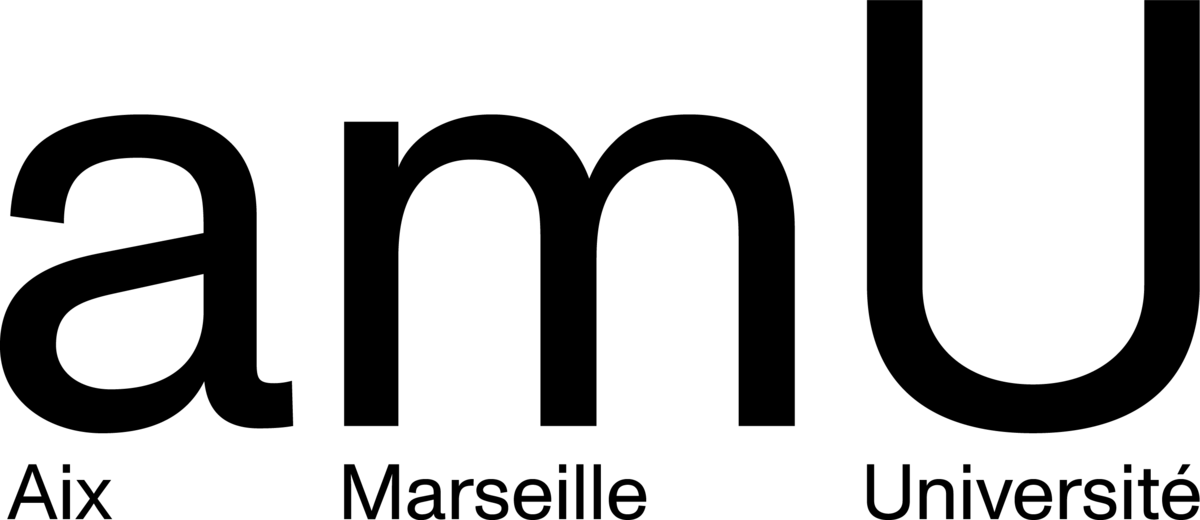
\includegraphics[scale=0.6]{images/LogoAMU.png}\hspace*{2cm}
	
\includegraphics[scale=0.2]{images/LogoCNRS.eps}\hspace*{2cm}
	
\includegraphics[scale=0.1]{images/LogoISM.eps}
\end{frame}

\section{Rappels de Mathématique} 
\subsection{Nombres complexes}

\begin{frame}
\begin{block}{Pourquoi des rappels sur les complexes ?}
\justifying
\textbf{\textcolor{red}{Les complexes}} sont utilisés dans pratiquement toutes
les sciences et \textbf{\textcolor{red}{tout particulièrement en traitement du
signal}} : représentation fréquentielles des signaux et des systèmes
\end{block}
\pause
\begin{block}{Pourquoi les complexes ?}
	\itemize
	  \item Résoudre certains problèmes insolubles autrement
	  \item Faciliter les calculs
\end{block}
\center
\begin{figure}[hbp]
\begin{center}
  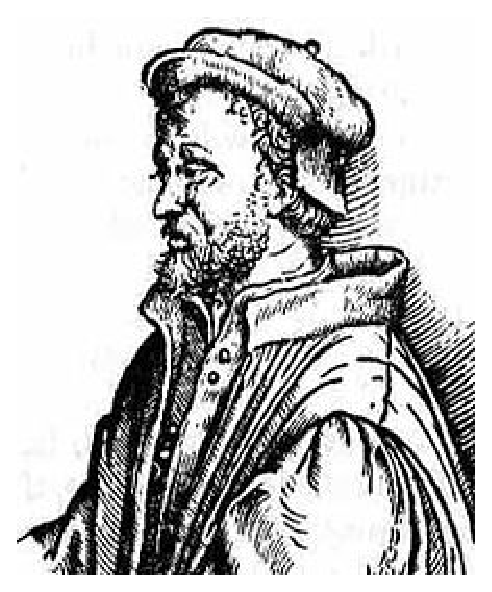
\includegraphics[scale=.25]{images/Cardano.eps}\\
  Jérôme CARDAN (1501-1576)
\end{center}
\end{figure}
\end{frame}

\begin{frame}
	\begin{block}{Le plan complexe}
		\begin{figure} 
			\psset{xunit=0.25cm}
			\psset{yunit=0.25cm}
			\begin{pspicture}[showgrid=false](-7,-7)(7,7)
				\psaxes[labels=none,ticks=none]{->}(-5,-5)(-7,-7)(7,5.25)
				\rput(-5,6.25){$\Im$}
				\rput(0.75,6.25){\tiny (axe des imaginaires purs)}
				\rput(7.75,-5){$\Re$}
				\rput(7.75,-6.25){\tiny (axe des réels)}
				\rput(-5,6.25){$\Im$}
				\psdot*[linecolor=red](-1,3)
				\psline[linecolor=black,linestyle=dashed](-1,3)(-1,-5)
				\psline[linecolor=black,linestyle=dashed](-1,3)(-5,3)
				\rput(1,4){\textcolor{red}{$M(z)$}}
				\rput(-1,-6){\textcolor{red}{$a$}}
				\rput(-6,3){\textcolor{red}{$b$}}
				\rput(-3.5,0){\textcolor{red}{$\rho$}}
				\psarc[linecolor=red,arcsepB=2pt,linewidth=1pt]{->}(-5,-5){0.7}{0}{65}
				\rput(-2,-3){\textcolor{red}{$\theta$}}
				\rput(-5.75,-5.75){$O$}
				\psline[linecolor=red](-5,-5)(-1,3)
				\psline[linecolor=black]{->}(-5,-5)(-3,-5)
				\psline[linecolor=black]{->}(-5,-5)(-5,-3)
				\rput(-4,-6){$\vec{e_{1}}$}
				\rput(-6,-4){$\vec{e_{2}}$}
			\end{pspicture}
		\end{figure} 
		$(O,\vec{e_{1}},\vec{e_{2}})$ est un repère orthonormé\\ 
		$\rho$ est la longueur du segment $[OM]$\\
		$\theta$ est l'angle orienté entre l'axe réel et la droite $(OM)$\\
		Le point $M$ est l'\textbf{image} du nombre complexe $z$\\
		$z$ est appelé \textbf{affixe} du point M\\
	\end{block}				
\end{frame}

\begin{frame}
\begin{columns}[t]
	\begin{column}{5.5cm}
		\begin{block}{Forme cartésienne}
			\[
			z = a + ib,\enspace i^{2}=-1
			\]
		\end{block}
		\pause
		\begin{block}{Forme polaire}
		\[
			z = \rho [cos(\theta) + isin(\theta)]
			\]
		\end{block}	
		\pause
	\end{column}
	\begin{column}{5.5cm}
		\begin{block}{Formule d'Euler}
			\[
			e^{i\theta} = cos(\theta) + isin(\theta)
			\]
		\end{block}
		\pause
		\begin{block}{Forme exponentielle}
			\[
			z = \rho e^{i\theta}
			\]
		\end{block}
	\end{column}
\end{columns}
\pause
\begin{columns}[t]
	\begin{column}{5.5cm}
		\begin{block}{Conjugué d'un nombre complexe}
			\begin{align*}
				\overline{z} &= a-ib\\
							&=\rho[cos(\theta) - isin(\theta)]\\
							&=\rho e^{-i\theta}
			\end{align*}
		\end{block}
	\end{column}
	\begin{column}{5.5cm} 
		\pause
		\begin{block}{Combinaison linéaire}
			\[
			Z =\alpha_1 z_1 + \alpha_2 z_2 + \alpha_3 z_3 + \alpha_4 z_4 \ldots
			\]
			\justifying
			$Z$ est un nombre complexe résultant de la somme pondérée de nombres complexes
		\end{block}
	\end{column}
\end{columns}
\end{frame}

\begin{frame} 
	\begin{exampleblock}{Exercice \Roman{exampleBlockCounter} -  Nombres complexes}
		\begin{enumerate}\justifying
			  \item Exprimer $\rho$ et $\theta$ en fonction de $a$ et $b$
			  \item Calculer $z \overline{z}$
			  \item Soit $z_1=2+5i$ sous forme cartésienne. Exprimer $z_1$ sous forme
			  polaire puis exponentielle
			  \item Soit $z_2=10e^{i\frac{\pi}{4}}$ sous forme exponentielle. Exprimer
			  $z_2$ sous forme polaire puis cartésienne.
			  \item Soit deux complexes $z_3$ et $z_4$, le premier réel pur de module
			  $4$ et le second imaginaire pur de module $5$. Exprimer $z_3$ et $z_4$
			  sous forme cartésienne puis exponentielle.
			  \item Exprimer les conjugués de tous ces nombres complexes sous forme
			  cartésienne et exponentielle.
			  \item Placer tous ces nombres dans la plan complexe.
			  \item Calculer $z_1z_2$, $\frac{z_1}{z_2}$, $z_3z_4$ et $\frac{z_1}{z_4}$
			  en utilisant la notation (cartésienne ou exponentielle) la plus appropriée.
		\end{enumerate}
	\end{exampleblock}\stepcounter{exampleBlockCounter}
\end{frame}
\begin{frame}
	\begin{exampleblock}{Exercice \Roman{exampleBlockCounter} - Nombres complexes avec Python}
		\begin{enumerate}\justifying
			  \item Définir les complexes $z_1$ (cartésienne), $z_2$ (exponentielle),
			  $z_3$ et $z_4$
			  \item En utilisant la commande \textit{\textcolor{red}{help}}, lire l'aide
			  des fonctions \textit{\textcolor{red}{real}},
			  \textit{\textcolor{red}{imag}}, \textit{\textcolor{red}{abs}},
			  \textit{\textcolor{red}{angle}} et \textit{\textcolor{red}{conj}}
			  \item En déduire le module et l'argument (la phase) de $z_1$. Vérifier le
			  résultat.
			  \item En déduire les parties réelles et imaginaires de $z_2$. Vérifier le
			  résultat.
			  \item Vérifiez les résultats obtenus aux questions six et huit de
			  l'exercice précédent.
			  \item Tracer ces nombres dans le même plan complexe en utilisant l'aide de
			  la fonction \textit{\textcolor{red}{plot}}
		\end{enumerate}
	\end{exampleblock}\stepcounter{exampleBlockCounter}
\end{frame}
\begin{frame}
	\begin{exampleblock}{Exercice \Roman{exampleBlockCounter} - Formule d'Euler}
		\begin{enumerate}\justifying
			  \item En partant de la formule d'Euler, montrer que $cos(\theta)
			  =\frac{e^{i\theta} + e^{-i\theta}}{2}$ et $sin(\theta)
			  =\frac{e^{i\theta} - e^{-i\theta}}{2i}$
			  \item En utilisant les résultats précédents, exprimer $cos^{2}(\theta)$ en
			  fonction de $cos(2\theta)$
			  \item De même, exprimer $sin^{2}(\theta)$ en
			  fonction de $cos(\theta)$ et $sin(\theta)$
		\end{enumerate}
	\end{exampleblock}\stepcounter{exampleBlockCounter}
\end{frame}

 
\end{document}